\chapter{Le sol vivant}\label{ch:b2:living-soil}

Le dernier livre de Charles Darwin, publié l'année précédant sa mort,
portait sur les \omterm{prop:b2:living-soil:community}{vers de terre}. Il avait répandu de la craie comme repère
sur un champ proche de sa maison en 1842 et l'avait déterrée en 1871~:
elle se trouvait à dix-huit centimètres de profondeur, enfouie sous les
turricules que les vers avaient remontés à la surface à un rythme qu'il
mesura, pesa et extrapola --- dix tonnes de terre par acre et par an
passant par leur corps, si bien que «~toute la terre végétale
superficielle d'une telle étendue est passée, et passera de nouveau, tous
les quelques ans, par le corps des vers~». Le \omterm{def:b2:living-soil:soil}{sol}, autrement dit, n'est
pas un support sur lequel se tiennent les êtres vivants, mais une chose
que les êtres vivants fabriquent. Ce chapitre traite de cette
fabrication~: comment la roche devient \omterm{def:b2:living-soil:soil}{sol}, et avec quelle lenteur, qui
y vit et en quel nombre, comment la matière morte est démontée et ce
qu'il en reste, comment les racines des plantes négocient avec des
champignons et des bactéries ce qu'elles ne peuvent obtenir seules, et à
quelle vitesse un \omterm{def:b2:living-soil:soil}{sol} qui a mis dix mille ans à se construire peut être
perdu.

\section{Ce qu'est le sol}

\begin{definition}[Le sol et ses horizons]\label{def:b2:living-soil:soil}
\index{sol}\index{horizon du sol}\index{humus}\index{alteration@altération}\index{pedogenese@pédogenèse}
Le \emph{sol} est la couche de matière minérale altérée, de matière
organique, d'eau, d'air et d'organismes qui recouvre les terres et porte
les plantes~: environ la moitié de son volume est formée de pores, remplis
d'eau ou d'air en proportions variables, et la moitié solide de grains
minéraux ---
sables (\qtyrange{0.05}{2}{mm}), limons (\qtyrange{2}{50}{\micro m}) et
argiles (moins de \qty{2}{\micro m}), dont les proportions donnent la
\emph{texture} --- avec quelques pour cent de matière organique qui
gouvernent l'essentiel de ses propriétés. Un profil de sol montre des
\emph{horizons}~: l'horizon \emph{O} de litière et de matière organique
partiellement décomposée, en surface~; l'horizon \emph{A}, sombre, de sol
minéral mêlé d'\emph{humus}, le résidu stable, sombre et colloïdal de la
décomposition~; l'horizon \emph{B} en dessous, vers lequel l'argile, le
fer et les matières dissoutes sont entraînés et où ils s'accumulent~;
l'horizon \emph{C} de roche mère altérée~; et la roche en place. Un sol
se forme (\emph{pédogenèse}) sous l'effet de cinq facteurs --- roche
mère, climat, organismes, topographie et temps --- et il se forme
lentement~: l'altération produit de l'ordre de \qty{0.1}{mm} de sol par
an, si bien qu'un mètre de sol représente dix mille ans de travail.
\end{definition}

\begin{omfigure}
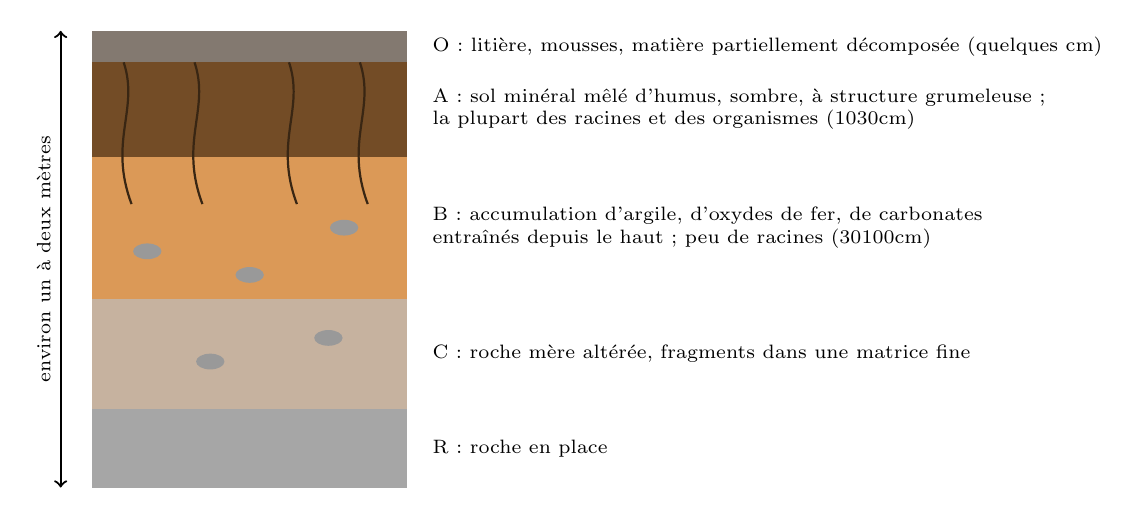
\begin{tikzpicture}[every node/.style={font=\scriptsize}]
  \fill[brown!25!black!60] (0,5.4) rectangle (4,5.8); \node[right] at (4.2,5.6) {O~: litière, mousses, matière partiellement décomposée (quelques cm)};
  \fill[brown!60!black] (0,4.2) rectangle (4,5.4); \node[right, align=left] at (4.2,4.8) {A~: sol minéral mêlé d'humus, sombre, à structure grumeleuse~;\\ la plupart des racines et des organismes (\qtyrange{10}{30}{cm})};
  \fill[brown!70!orange!80] (0,2.4) rectangle (4,4.2); \node[right, align=left] at (4.2,3.3) {B~: accumulation d'argile, d'oxydes de fer, de carbonates\\ entraînés depuis le haut~; peu de racines (\qtyrange{30}{100}{cm})};
  \fill[gray!50!brown!60] (0,1.0) rectangle (4,2.4); \node[right, align=left] at (4.2,1.7) {C~: roche mère altérée, fragments dans une matrice fine};
  \fill[gray!70] (0,0) rectangle (4,1.0); \node[right] at (4.2,0.5) {R~: roche en place};
  \foreach \x in {0.4,1.3,2.5,3.4} \draw[brown!30!black, thick] (\x,5.4) .. controls (\x+0.2,4.8) and (\x-0.2,4.4) .. (\x+0.1,3.6);
  \foreach \x/\y in {0.7/3.0, 2.0/2.7, 3.2/3.3, 1.5/1.6, 3.0/1.9} \fill[gray!80] (\x,\y) ellipse (0.18 and 0.1);
  \draw[<->, thick] (-0.4,5.8) -- (-0.4,0) node[midway, left, rotate=90, anchor=south] {environ un à deux mètres};
\end{tikzpicture}

{\small Un profil de \omterm{def:b2:living-soil:soil}{sol}. La matière organique entre par le haut et est
consommée à mesure qu'elle descend~; la matière minérale est libérée par
le bas et remontée par les racines et les animaux~; les matières dissoutes
descendent avec l'eau et sont retenues dans l'horizon B.}
\end{omfigure}

\begin{proposition}[Pourquoi l'argile et l'humus comptent]\label{prop:b2:living-soil:cec}
\index{capacite d'echange cationique@capacité d'échange cationique}\index{argile}\index{structure du sol}\index{capacite au champ@capacité au champ}
Les particules d'argile et l'\omterm{def:b2:living-soil:soil}{humus} portent des charges négatives à leur
surface et retiennent, par attraction électrostatique, une réserve de
cations échangeables --- $\mathrm{Ca^{2+}}$, $\mathrm{Mg^{2+}}$, $\mathrm{K^{+}}$, $\mathrm{NH_4^{+}}$ --- dans
laquelle les racines puisent en les échangeant contre des $\mathrm{H^{+}}$. Cette
\emph{\omterm{prop:b2:living-soil:cec}{capacité d'échange cationique}} est la banque de nutriments du \omterm{def:b2:living-soil:soil}{sol}~;
un sable n'en a presque pas (quelques centimoles de charge par
kilogramme), un limon argileux riche en \omterm{def:b2:living-soil:soil}{humus} cinquante fois plus, et la
fertilité des deux diffère en conséquence. Les mêmes surfaces retiennent
l'eau~: un \omterm{def:b2:living-soil:soil}{sol} sableux se ressuie en une journée jusqu'à une
\emph{\omterm{prop:b2:living-soil:cec}{capacité au champ}} d'un dixième de son volume, un limon en retient
un tiers, et la différence est ce dont dispose une culture entre deux
pluies. Enfin, l'\omterm{def:b2:living-soil:soil}{humus}, avec les hyphes des champignons, les exsudats
racinaires et le mucus des vers, colle les grains minéraux en
\emph{agrégats}, la structure grumeleuse dont les pores laissent passer
l'air, l'eau et les racines --- la propriété qui distingue un \omterm{def:b2:living-soil:soil}{sol} d'un
sédiment, et la première que détruisent le labour et le tassement.
\end{proposition}

\section{Qui y vit}

\begin{proposition}[La communauté du sol]\label{prop:b2:living-soil:community}
\index{reseau trophique du sol@réseau trophique du sol}\index{detritivore@détritivore}\index{ver de terre}\index{biomasse du sol}
Un gramme de terre arable fertile contient environ $10^{9}$ cellules
bactériennes d'une dizaine de milliers d'espèces, une centaine de mètres
d'hyphes fongiques, $10^{4}$
\omterm{def:b2:unicellular-diversity:protist}{protistes}, quelques dizaines de nématodes et une poignée d'acariens et de
collemboles~; un mètre carré contient quelques centaines de \omterm{prop:b2:living-soil:community}{vers de terre}
et, sous les animaux visibles, une masse vivante de plusieurs tonnes par
hectare --- comparable au bétail que le même hectare pourrait nourrir.
La communauté forme un \emph{réseau trophique détritique}~: bactéries et
champignons (les \emph{décomposeurs}) mangent la matière morte et sont
mangés par les \omterm{def:b2:unicellular-diversity:protist}{protistes} et les nématodes (les brouteurs de microbes),
eux-mêmes mangés par les acariens et les nématodes prédateurs, qui
nourrissent les chilopodes et les coléoptères~; les \emph{détritivores}
--- \omterm{prop:b2:living-soil:community}{vers de terre}, diplopodes, cloportes, termites, collemboles ---
mangent la litière elle-même avec les microbes qui la couvrent, la
fragmentant mille fois et multipliant la surface qu'attaquent les
microbes. Les brouteurs comptent au-delà de leur nombre~: en mangeant
les bactéries, ils libèrent sous forme d'ammonium l'azote immobilisé dans
les cellules bactériennes, et un \omterm{def:b2:living-soil:soil}{sol} pourvu de \omterm{def:b2:unicellular-diversity:protist}{protistes} et de nématodes
minéralise l'azote plus vite qu'un \omterm{def:b2:living-soil:soil}{sol} qui ne contient que des bactéries.
Les \omterm{prop:b2:living-soil:community}{vers de terre} sont les \emph{ingénieurs de l'écosystème}~: leurs
galeries sont les macropores du \omterm{def:b2:living-soil:soil}{sol}, leurs turricules les agrégats les
plus riches, et les vers d'une prairie font passer chaque année quelques
tonnes de terre par hectare dans leur tube digestif, comme l'avait
mesuré Darwin.
\end{proposition}

\begin{omfigure}
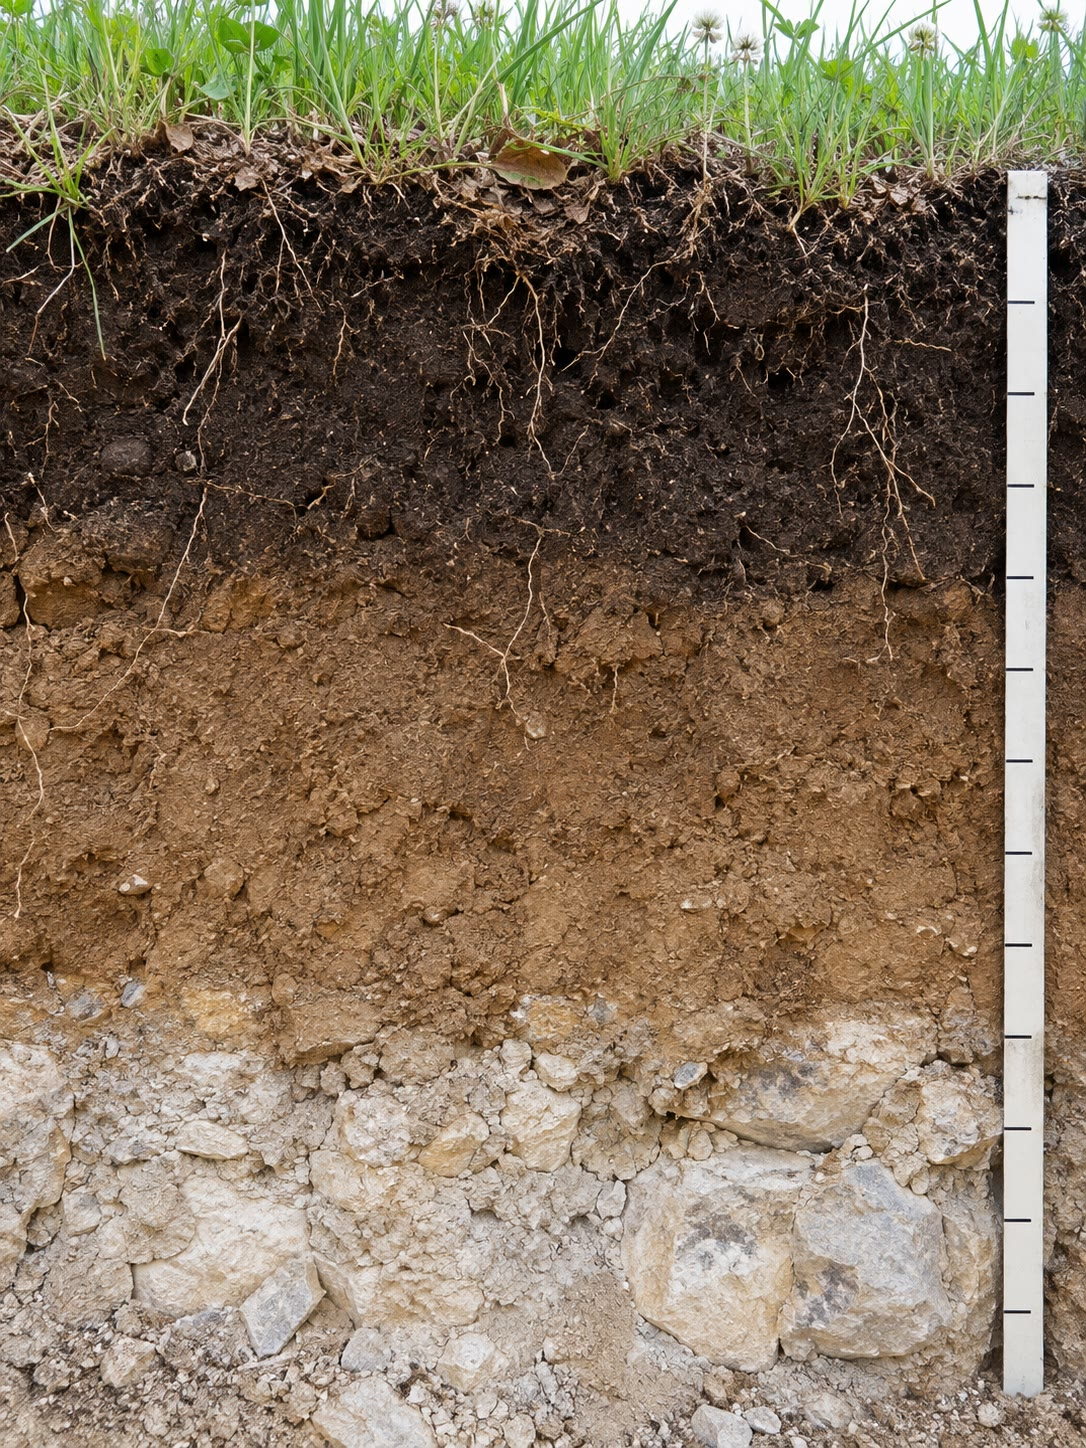
\includegraphics[width=0.21\linewidth]{images/book4/ai/b4-26-soil-profile.jpg}\hspace{0.025\linewidth}
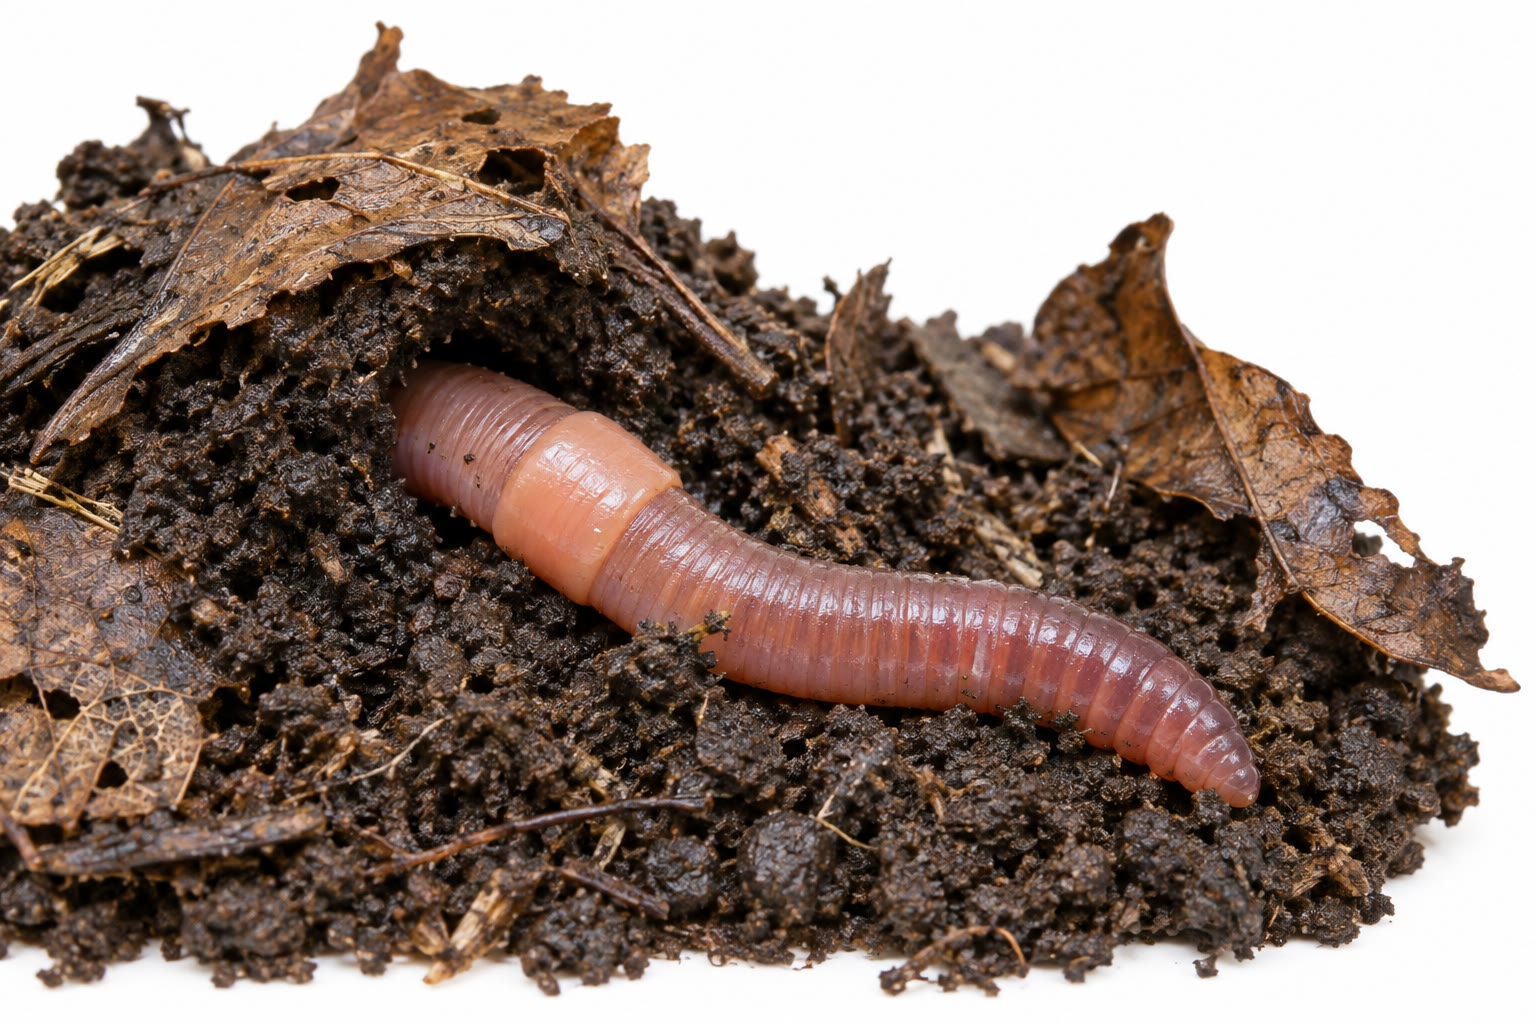
\includegraphics[width=0.42\linewidth]{images/book4/ai/b4-26-earthworm.jpg}\hspace{0.025\linewidth}
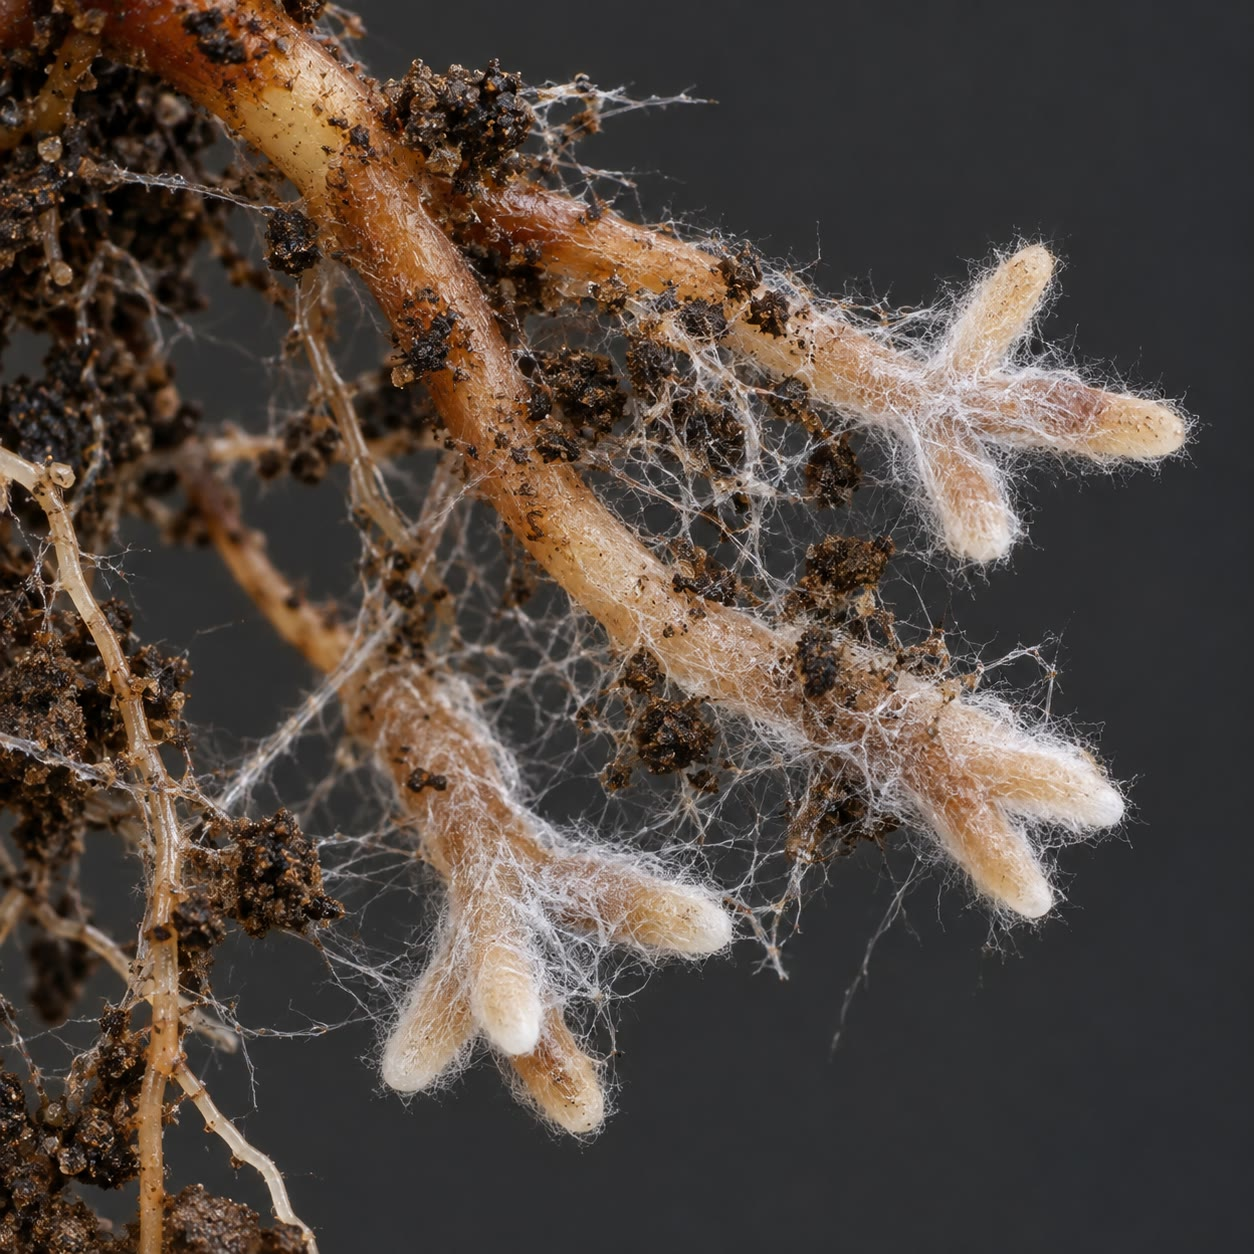
\includegraphics[width=0.28\linewidth]{images/book4/ai/b4-26-mycorrhiza.jpg}

{\small Le \omterm{def:b2:living-soil:soil}{sol} et deux de ses bâtisseurs. À gauche~: un profil dans un
talus, la terre arable sombre passant progressivement à la roche altérée
pâle. Au centre~: un \omterm{prop:b2:living-soil:community}{ver de terre} dans sa galerie. À droite~: une racine
avec son manchon ectomycorhizien et les hyphes qui la prolongent dans le
\omterm{def:b2:living-soil:soil}{sol}.}
\end{omfigure}

\section{La décomposition}

\begin{theorem}[La décomposition de la litière et le rapport carbone sur azote]\label{thm:b2:living-soil:decay}
\index{decomposition@décomposition}\index{decomposition de la litiere@décomposition de la litière}\index{rapport C:N}\index{mineralisation@minéralisation}\index{immobilisation}
La litière se décompose à une vitesse proportionnelle à ce qui reste,
$\mathrm{d}L/\mathrm{d}t = -kL$, donc $L = L_0 e^{-kt}$, avec une
\emph{constante de décomposition} $k$ d'environ 1 par an pour les herbes
et les feuilles caduques d'une forêt tempérée, $0.3$ pour les aiguilles
de conifères, plusieurs par an sous les tropiques humides et $0.05$ dans
la toundra~;
un apport constant $I$ par an construit une couche de litière de $I/k$. La
décomposition est contrôlée par la température, l'humidité et la
\emph{qualité} de la litière~: teneur en azote, teneur en lignine et
rapport du carbone à l'azote. Les microbes ont un $\mathrm{C:N} \approx 8$ et
retiennent environ \qty{40}{\%} du carbone qu'ils consomment~: il leur
faut donc un azote pour $8/0.4 = 20$ carbones de nourriture. Une litière de $\mathrm{C:N}$
inférieur à 25 environ libère de l'ammonium en se décomposant
(\emph{minéralisation}), tandis qu'une litière au-dessus de ce seuil ---
la paille à 80, le \omterm{def:b2:plant-meristems:wood}{bois} à 400 --- oblige les microbes à prélever l'azote
du \omterm{def:b2:living-soil:soil}{sol} (\emph{immobilisation}), affamant les plantes jusqu'à ce que le
carbone ait été respiré et que le rapport ait baissé. C'est pourquoi une
paille fraîche enfouie par le labour déprime une culture, pourquoi des
résidus de légumineuses la nourrissent, et pourquoi un tas de compost a
besoin des deux.
\end{theorem}
\begin{proof}
Pour le rapport~: des microbes qui consomment une litière comptant $c$
carbones par azote assimilent $0.4c$ carbones et, pour construire une
biomasse de
$\mathrm{C:N} = 8$, ont besoin de $0.4c/8 = c/20$ azotes~; la litière en
fournit 1. Si $c < 20$, l'azote est en excès et libéré sous forme
d'ammonium~; si $c > 20$, le déficit est prélevé dans le \omterm{def:b2:living-soil:soil}{sol}. Le seuil de
25 observé en pratique traduit une efficacité de rétention un peu
inférieure à 0.4. Pour la couche de litière~: $\mathrm{d}L/\mathrm{d}t = I - kL$
a pour \omterm{def:b2:biogeochemical-cycles:reservoir}{état stationnaire} $I/k$, atteint avec la constante de temps
$1/k$~; le \omterm{def:b2:biogeochemical-cycles:reservoir}{temps de résidence} de la litière vaut $1/k$, un an dans une
hêtraie et vingt ans dans la toundra.
\end{proof}
\begin{proof}[Faits expérimentaux]
Les expériences en sacs à litière --- des masses connues de feuilles dans
des sacs en filet, enfouis et pesés à intervalles réguliers --- ont donné
la loi exponentielle et ses constantes dans tous les biomes (Olson, 1963),
et ont montré, avec des mailles de tailles différentes, qu'exclure les
animaux du \omterm{def:b2:living-soil:soil}{sol} divise la vitesse par deux~: les microbes font la chimie,
mais les animaux donnent le rythme. À l'échelle d'un continent, la même
feuille se décompose en un an en Géorgie et en huit en Alaska, en
proportion de l'évapotranspiration réelle, produit de la chaleur et de
l'eau.
\end{proof}

\begin{omfigure}
\begin{tikzpicture}
\begin{axis}[
  width=0.72\linewidth, height=5.6cm,
  axis x line=bottom, axis y line=left,
  xmin=0, xmax=6, ymin=0, ymax=105,
  xlabel={années}, ylabel={masse de litière restante (\%)},
  xlabel style={font=\small, at={(axis description cs:0.5,-0.13)}, anchor=north},
  ylabel style={font=\small},
  tick label style={font=\small},
  legend style={font=\scriptsize, at={(0.5,-0.3)}, anchor=north, draw=none, legend columns=2},
  clip=false,
]
\addplot[very thick, omDef, domain=0:6, samples=60] {100*exp(-2*x)};
\addlegendentry{feuille de forêt tropicale, $k = 2$}
\addplot[very thick, omThm, domain=0:6, samples=60] {100*exp(-1*x)};
\addlegendentry{feuille de hêtre, $k = 1$}
\addplot[very thick, omProp, domain=0:6, samples=60] {100*exp(-0.3*x)};
\addlegendentry{aiguille d'épicéa, $k = 0.3$}
\addplot[very thick, gray, domain=0:6, samples=60] {100*exp(-0.05*x)};
\addlegendentry{mousse de toundra, $k = 0.05$}
\end{axis}
\end{tikzpicture}

{\small Décomposition exponentielle de la litière. La moitié d'une
feuille de hêtre a disparu en huit mois~; la moitié d'une \omterm{def:b2:plant-life-cycles:moss}{mousse} de
toundra en quatorze ans~; le résidu qu'aucun microbe ni aucun animal ne
peut achever devient de l'\omterm{def:b2:living-soil:soil}{humus}.}
\end{omfigure}

\begin{proposition}[L'humus et le réservoir de carbone du sol]\label{prop:b2:living-soil:humus}
\index{humus}\index{carbone organique du sol}\index{respiration du sol}
Quelques pour cent du carbone de la litière échappent à l'oxydation
complète et deviennent de l'\emph{\omterm{def:b2:living-soil:soil}{humus}}~: un mélange sombre et amorphe de
résidus microbiens, de lignine altérée et de composés végétaux, lié à
l'argile et au fer et enfermé dans les agrégats, qui se décompose avec des
\omterm{def:b2:biogeochemical-cycles:reservoir}{temps de résidence} allant de décennies à millénaires. C'est dans l'\omterm{def:b2:living-soil:soil}{humus}
que réside la fertilité du \omterm{def:b2:living-soil:soil}{sol}
--- l'essentiel de son azote et de sa capacité d'échange, la moitié de sa
rétention en eau --- et c'est le plus grand \omterm{def:b2:biogeochemical-cycles:reservoir}{réservoir} de carbone
organique des terres émergées,
\qty{1700}{GtC} dans le premier mètre, deux fois celui de l'atmosphère. Son
bilan est l'apport moins la décomposition, $\mathrm{d}H/\mathrm{d}t = I_h - k_hH$~:
avec $k_h \approx 0.02$ par an, un \omterm{def:b2:living-soil:soil}{sol} contient cinquante ans d'apport,
et toute modification --- le labour, qui brise les agrégats et aère
l'\omterm{def:b2:living-soil:soil}{humus}~; le drainage d'une tourbière, qui y fait entrer l'oxygène~; le
réchauffement, qui augmente $k_h$ --- se traduit par une perte qui se
poursuit pendant des décennies. Les \omterm{def:b2:living-soil:soil}{sols} cultivés du monde ont perdu d'un
tiers à la moitié de leur \omterm{def:b2:living-soil:soil}{humus} depuis leur première mise en culture,
quelque
\qty{100}{GtC}, et un réchauffement de \qty{3}{\celsius} accroîtrait d'un
tiers la décomposition du reste~: les \omterm{def:b2:living-soil:soil}{sols} sont la plus grande incertitude
du bilan carbone du \cref{ch:b2:global-change}.
\end{proposition}

\section{Les partenariats souterrains}

\begin{proposition}[Mycorhizes et rhizobiums]\label{prop:b2:living-soil:symbiosis}
\index{mycorhize}\index{rhizobium}\index{nodosite@nodosité}\index{nitrogenase@nitrogénase}\index{leghemoglobine@leghémoglobine}
Neuf espèces végétales sur dix ont des racines colonisées par des
champignons formant une
\emph{mycorhize}~: la plante fournit du sucre (d'un dixième à un
cinquième de ses photosynthétats) et le champignon fournit du phosphate,
de l'azote, de l'eau et du zinc, que ses hyphes, cent fois plus fines
qu'une racine et s'étendant sur cent fois sa longueur par unité de
carbone, récoltent dans un volume de \omterm{def:b2:living-soil:soil}{sol} que la racine ne peut atteindre
--- le phosphate en particulier, qui diffuse si lentement dans le \omterm{def:b2:living-soil:soil}{sol}
qu'une racine épuise en quelques jours le millimètre qui l'entoure.
Les mycorhizes \emph{arbusculaires}, les plus anciennes, pénètrent dans
les cellules de la racine et s'y ramifient en arbuscules où ont lieu les
échanges~; les \emph{ectomycorhizes} des arbres forestiers engainent
l'extrémité de la racine et se développent entre ses cellules. Les
légumineuses vont plus loin~: les rhizobiums, attirés par les flavonoïdes
de la racine, entrent par un \omterm{prop:b2:plant-meristems:ram}{poil absorbant}, et la racine construit
autour d'eux une \emph{nodosité} dans laquelle les bactéries, devenues
\emph{bactéroïdes}, fixent l'azote grâce à la nitrogénase --- une enzyme
si sensible à l'oxygène que la nodosité doit être maintenue presque
anoxique par la
\emph{leghémoglobine}, une hémoglobine fabriquée par la plante, qui donne
à la nodosité sa couleur rose et délivre l'oxygène aux bactéroïdes à une
concentration trop faible pour empoisonner l'enzyme. Chaque partenaire
surveille l'autre~: une plante coupe le sucre aux nodosités qui ne fixent
rien, et un champignon qui délivre moins de phosphate reçoit moins de
carbone.
\end{proposition}
\begin{proof}[Faits expérimentaux]
Kiers et ses collègues (2011) cultivèrent une plante associée à deux
partenaires fongiques sur un système racinaire divisé et n'offrirent du
phosphate que d'un côté~: la plante attribua davantage de carbone au
champignon qui fournissait le plus de phosphate, et le champignon
attribua davantage de phosphate à la racine qui donnait le plus de
carbone --- des récompenses réciproques mesurées à l'aide d'isotopes.
Chez les rhizobiums, des nodosités privées expérimentalement d'azote (en
remplaçant l'air par un mélange d'argon et d'oxygène) recevaient moins
d'oxygène et grandissaient moins que les nodosités de la même plante
capables de fixer~: la plante sanctionne les tricheurs. Le traçage à
l'azote 15 montre qu'une prairie de trèfle et de graminées transfère aux
graminées un tiers de l'azote fixé par le trèfle en une saison, par le
\omterm{def:b2:living-soil:soil}{sol} et par des réseaux fongiques partagés.
\end{proof}

\begin{omfigure}
\begin{tikzpicture}[every node/.style={font=\scriptsize}, >=stealth]
  % root cross-section
  \fill[omThm!15] (0,0) circle (1.5); \draw[thick] (0,0) circle (1.5);
  \fill[omThm!30] (0,0) circle (0.5); \draw[thick] (0,0) circle (0.5);
  \node at (0,0) {stèle};
  \node at (0,1.05) {cortex};
  % arbuscules in cortex cells
  \foreach \a in {30,150,270} { \draw[omDef, thick] ({1.0*cos(\a)},{1.0*sin(\a)}) -- ++({0.25*cos(\a+60)},{0.25*sin(\a+60)}) -- ++({0.2*cos(\a-40)},{0.2*sin(\a-40)}); \draw[omDef, thick] ({1.0*cos(\a)},{1.0*sin(\a)}) -- ++({0.25*cos(\a-60)},{0.25*sin(\a-60)}); }
  % hyphae out
  \foreach \a in {20,80,150,210,340} { \draw[omDef, thick] ({1.5*cos(\a)},{1.5*sin(\a)}) .. controls ({2.2*cos(\a+10)},{2.2*sin(\a+10)}) .. ({2.7*cos(\a-5)},{2.7*sin(\a-5)}); }
  \draw[omDef, thick] ({1.5*cos(150)},{1.5*sin(150)}) -- ({1.0*cos(150)},{1.0*sin(150)});
  \node[omDef, anchor=west, align=left] at (2.9,1.4) {hyphes~: \qty{3}{\micro m} de large,\\ des mètres par centimètre de racine};
  \node[omDef, anchor=west] at (2.9,0.1) {arbuscule dans une cellule du cortex};
  \draw[omDef] (2.85,0.1) -- (1.2,0.5);
  \node[anchor=north, align=center] at (0,-1.6) {racine, \qty{0.3}{mm} de diamètre};
  \draw[->, thick, omThm] (-1.2,-2.4) -- (1.2,-2.4) node[right] {sucre vers le champignon, \qtyrange{10}{20}{\%} des photosynthétats};
  \draw[<-, thick, omDef] (-1.2,-2.9) -- (1.2,-2.9) node[right] {phosphate, ammonium, eau, zinc vers la plante};
  % nodule
  \begin{scope}[xshift=9.3cm]
    \draw[thick, brown!60!black] (-0.3,2.4) -- (-0.1,-0.6);
    \draw[thick, brown!60!black] (-0.1,0.3) -- (1.6,0.1);
    \fill[pink!60!red!40] (1.5,0.2) circle (0.9); \draw[thick] (1.5,0.2) circle (0.9);
    \fill[pink!80!red!60] (1.5,0.2) circle (0.55);
    \foreach \p in {(1.3,0.3),(1.6,0.0),(1.5,0.45),(1.7,0.3),(1.35,0.05)} \fill[omDef!70!black] \p ellipse (0.08 and 0.05);
    \node[anchor=north, align=center] at (1.5,-0.8) {nodosité~: bactéroïdes dans les cellules,\\ rose de leghémoglobine~;\\ oxygène maintenu à \qty{10}{nM}~: la nitrogénase\\ fonctionne et les cellules respirent};
    \node[anchor=south, align=center] at (-0.2,2.45) {racine de légumineuse};
  \end{scope}
\end{tikzpicture}

{\small Deux marchés. À gauche~: une mycorhize arbusculaire, le sucre
sortant et le phosphate entrant par les arbuscules situés dans les
cellules du cortex. À droite~: une nodosité de légumineuse, où
l'hémoglobine propre de la plante maintient l'oxygène assez bas pour la
nitrogénase et assez haut pour la respiration.}
\end{omfigure}

\section{Perdre le sol}

\begin{proposition}[Érosion, sel et bilan d'un sol]\label{prop:b2:living-soil:erosion}
\index{erosion des sols@érosion des sols}\index{salinisation}\index{desertification@désertification}
Le \omterm{def:b2:living-soil:soil}{sol} se forme à raison de \qtyrange{0.05}{0.5}{mm} par an et, sous une
végétation naturelle, s'érode à peu près au même rythme. Une terre nue
labourée en pente perd \qtyrange{1}{10}{mm} par an sous l'effet de l'eau
et du vent ---
\qtyrange{10}{100}{t/ha} --- dix à cent fois la vitesse de formation~: un
\omterm{def:b2:living-soil:soil}{sol} construit en dix mille ans disparaît en un siècle, et avec lui
l'\omterm{def:b2:living-soil:soil}{humus} et les nutriments de l'horizon A, la seule partie qui compte.
Les cultures intermédiaires, les terrasses, le labour en courbes de
niveau et le semis direct, qui laisse les résidus en surface et les
agrégats intacts, ramènent la perte près de la vitesse de formation.
L'irrigation en climat sec provoque l'échec inverse~: l'eau s'évapore et
laisse ses sels, une tonne par hectare et par an à partir d'une eau à
peine saline, jusqu'à ce que le potentiel osmotique de la solution du \omterm{def:b2:living-soil:soil}{sol}
(\cref{ch:b2:plant-plasticity}) soit plus bas que ce que les racines
peuvent surmonter --- la \emph{salinisation}, qui fit abandonner les
champs de Sumer il y a quatre mille ans et touche aujourd'hui un
cinquième des terres irriguées. L'état d'un \omterm{def:b2:living-soil:soil}{sol} est un bilan~: \omterm{def:b2:living-soil:soil}{humus}
entrant contre \omterm{def:b2:living-soil:soil}{humus} sortant, formation contre érosion, sel apporté
contre sel drainé~; chacun a un \omterm{def:b2:biogeochemical-cycles:reservoir}{temps de résidence}, et chacun, une fois
négatif, est lent à inverser.
\end{proposition}

\section{Exercices}

\begin{exercise}[$\star$]\label{exo:b2:living-soil:1}
Nommer les horizons d'un profil de \omterm{def:b2:living-soil:soil}{sol}, de la surface vers la
profondeur, et dire ce qui se passe dans chacun.
\end{exercise}

\begin{exercise}[$\star$]\label{exo:b2:living-soil:2}
Expliquer ce qu'est la \omterm{prop:b2:living-soil:cec}{capacité d'échange cationique}, pourquoi un \omterm{def:b2:living-soil:soil}{sol}
sableux en a peu, et ce que fait à un \omterm{def:b2:living-soil:soil}{sol} acide un agriculteur qui le
chaule.
\end{exercise}

\begin{exercise}[$\star$]\label{exo:b2:living-soil:3}
Énumérer les principaux groupes du \omterm{prop:b2:living-soil:community}{réseau trophique du sol}, des
décomposeurs aux prédateurs supérieurs, avec un organisme pour chacun, et
dire ce que les brouteurs de bactéries apportent aux plantes.
\end{exercise}

\begin{exercise}[$\star$]\label{exo:b2:living-soil:4}
Distinguer mycorhizes arbusculaires et ectomycorhizes, et préciser ce
que chaque partenaire donne et reçoit.
\end{exercise}

\begin{exercise}[$\star\star$]\label{exo:b2:living-soil:5}
Une hêtraie laisse tomber \qty{4}{t/ha} de feuilles par an et la
\omterm{thm:b2:living-soil:decay}{décomposition de la litière} suit $k = 0.8$ par an. Calculer la masse de litière à l'\omterm{def:b2:biogeochemical-cycles:reservoir}{état
stationnaire}, le \omterm{def:b2:biogeochemical-cycles:reservoir}{temps de résidence} de la litière, et le temps nécessaire
pour que la chute d'une année perde \qty{90}{\%} de sa masse.
\end{exercise}

\begin{exercise}[$\star\star$]\label{exo:b2:living-soil:6}
La paille de blé a un $\mathrm{C:N} = 80$ et les résidus de trèfle $15$.
Pour chacun, calculer l'azote dont les microbes ont besoin pour
\qty{100}{kg} de carbone consommé (rétention 0.4, $\mathrm{C:N} = 8$ pour les
microbes) et dire si le résidu minéralise ou immobilise l'azote, et en quelle
quantité.
\end{exercise}

\begin{exercise}[$\star\star$]\label{exo:b2:living-soil:7}
Un hectare de prairie contient \qty{2}{t} de \omterm{prop:b2:living-soil:community}{vers de terre}, qui font
chacun passer chaque année dix fois leur masse de terre. Calculer la
terre qui passe par les vers en un an et le temps nécessaire pour que les
\qty{20}{cm} supérieurs (masse volumique apparente \qty{1.3}{t/m^3}) y
passent une fois. Comparer au chiffre de Darwin.
\end{exercise}

\begin{exercise}[$\star\star$]\label{exo:b2:living-soil:8}
Un gramme de \omterm{def:b2:living-soil:soil}{sol} contient $10^{9}$ bactéries de \qty{e-12}{g} chacune, et
\qty{100}{m} d'hyphes de \qty{4}{\micro m} de diamètre et de masse
volumique \qty{1.1}{g/cm^3}. Calculer la biomasse bactérienne et fongique
par gramme et par hectare (\qty{20}{cm} supérieurs, \qty{1.3}{t/m^3}).
\end{exercise}

\begin{exercise}[$\star\star$]\label{exo:b2:living-soil:9}
L'\omterm{def:b2:living-soil:soil}{humus} du \omterm{def:b2:living-soil:soil}{sol} se décompose avec $k_h = 0.02$ par an et reçoit
\qty{1.5}{t/ha} de carbone par an. Calculer le carbone de l'\omterm{def:b2:living-soil:soil}{humus} à
l'\omterm{def:b2:biogeochemical-cycles:reservoir}{état stationnaire}. Le champ est labouré et $k_h$ double~: calculer le
nouvel \omterm{def:b2:biogeochemical-cycles:reservoir}{état stationnaire}, le carbone perdu et le temps nécessaire pour en
perdre la moitié.
\end{exercise}

\begin{exercise}[$\star\star\star$]\label{exo:b2:living-soil:10}
Le phosphate diffuse dans le \omterm{def:b2:living-soil:soil}{sol} avec $D \approx \qty{e-13}{m^2/s}$.
Calculer la distance qu'il parcourt en une saison de croissance de
\num{100} jours ($x \approx \sqrt{2Dt}$) et la comparer à l'espacement
des racines (\qty{1}{cm}) et des hyphes (\qty{0.1}{mm}). Qu'est-ce que
cela dit de la raison pour laquelle les mycorhizes comptent pour le
phosphore, et moins pour le nitrate ($D \approx \qty{e-10}{m^2/s}$)~?
\end{exercise}

\begin{exercise}[$\star\star\star$]\label{exo:b2:living-soil:11}
Une pente perd \qty{20}{t/ha} de terre par an par érosion tout en en
formant \qty{1}{t/ha}~; l'horizon A a une épaisseur de \qty{25}{cm}, à
\qty{1.3}{t/m^3}, et contient \qty{3}{\%} de carbone. Calculer la masse
de l'horizon A, sa durée de vie à ce rythme et le carbone perdu par an.
En semis direct, la perte tombe à \qty{2}{t/ha}~: recalculer la durée de
vie.
\end{exercise}

\begin{exercise}[$\star\star\star$]\label{exo:b2:living-soil:12}
«~Le \omterm{def:b2:living-soil:soil}{sol} est l'organisme le plus lent de la ferme.~» Discuter à l'aide
des \omterm{def:b2:biogeochemical-cycles:reservoir}{temps de résidence} de la litière, de l'\omterm{def:b2:living-soil:soil}{humus}, du \omterm{def:b2:living-soil:soil}{sol} minéral et du
sel, et dire quels changements un agriculteur peut voir au cours de sa
carrière et lesquels non.
\end{exercise}

\section{Problème~: un hectare de sol}

\begin{problem}[{Problème du week-end --- l'audit d'un hectare de sol
cultivé~: sa masse vivante dénombrée, sa litière et son humus suivis à
travers leurs bilans exponentiels, l'azote libéré par un résidu de
légumineuse confronté aux besoins d'une culture, et les bilans d'érosion
et de carbone de deux modes de conduite comparés, jusqu'au stock de
carbone du sol, à sa durée de vie sous le labour et à l'azote que fournit
une légumineuse}]
\label{pb:b2:living-soil:1}
L'hectare~: horizon A de \qty{25}{cm} d'épaisseur, masse volumique
apparente \qty{1.3}{t/m^3}, \qty{2.5}{\%} de carbone organique~;
décomposition de l'\omterm{def:b2:living-soil:soil}{humus} $k_h =
0.025$ par an sous le labour, $0.015$ en semis direct~; apport de carbone
à l'\omterm{def:b2:living-soil:soil}{humus} \qty{1.2}{t/ha} par an dans les deux cas. Litière~: une culture
intermédiaire de trèfle laisse \qty{5}{t/ha} de matière sèche à
\qty{45}{\%} de carbone et \qty{3}{\%} d'azote, qui se décompose avec $k = 2$
par an. Érosion~: \qty{15}{t/ha} par an sous le labour, \qty{1.5}{t/ha}
en semis direct~; formation \qty{0.5}{t/ha}.

\medskip
\noindent\textbf{Partie I --- Le stock.}
\begin{enumerate}
  \item Calculer la masse de l'horizon A et son carbone organique.
  \item Calculer la masse d'azote de l'\omterm{def:b2:living-soil:soil}{humus} si son
        $\mathrm{C:N}$ vaut 12.
  \item Le \omterm{def:b2:living-soil:soil}{sol} contient $10^{9}$ bactéries par gramme, de \qty{e-12}{g}
        chacune, et \qty{200}{m} d'hyphes par gramme, de \qty{4}{\micro m}
        de diamètre et de masse volumique 1.1. Calculer la biomasse
        microbienne par hectare.
  \item Ajouter \qty{1.5}{t/ha} de \omterm{prop:b2:living-soil:community}{vers de terre} et \qty{0.2}{t/ha}
        d'autres animaux, et donner la masse vivante totale par hectare.
        Quelle fraction du carbone de l'\omterm{def:b2:living-soil:soil}{humus} représente-t-elle~?
  \item Les microbes renouvellent leur biomasse deux fois par an et
        respirent \qty{60}{\%} de ce qu'ils consomment. Estimer le carbone
        qu'ils consomment par an, et le $\mathrm{CO_2}$ respiré.
  \item Comparer à la production primaire nette de la culture, environ
        \qty{5}{t/ha} de carbone, et commenter.
\end{enumerate}

\medskip
\noindent\textbf{Partie II --- Le résidu de trèfle.}
\begin{enumerate}[resume]
  \item Calculer le carbone et l'azote du résidu et son
        $\mathrm{C:N}$.
  \item Avec $\mathrm{C:N} = 8$ pour les microbes et une rétention de $0.4$,
        le résidu minéralise-t-il ou immobilise-t-il l'azote~? Calculer
        l'azote net libéré par la décomposition de tout le résidu.
  \item Avec $k = 2$, quelle fraction du résidu s'est décomposée au bout
        de 3 mois~? D'un an~?
  \item Calculer l'azote libéré pendant les 3 premiers mois.
  \item Une culture de blé prélève \qty{150}{kg} d'azote par hectare,
        pour l'essentiel dans les deux mois qui suivent le semis.
        Commenter le calendrier.
  \item On enfouit à la place la même masse de paille de blé
        ($\mathrm{C:N} = 80$). Calculer l'azote immobilisé et dire ce que
        l'agriculteur doit faire.
\end{enumerate}

\medskip
\noindent\textbf{Partie III --- L'\omterm{def:b2:living-soil:soil}{humus}.}
\begin{enumerate}[resume]
  \item Calculer le carbone de l'\omterm{def:b2:living-soil:soil}{humus} à l'\omterm{def:b2:biogeochemical-cycles:reservoir}{état stationnaire} sous le
        labour et en semis direct.
  \item Le champ, à l'\omterm{def:b2:biogeochemical-cycles:reservoir}{état stationnaire} du labour, passe au semis direct.
        Écrire $H(t)$ et calculer le carbone gagné au bout de 10 et de
        50 ans.
  \item Calculer la vitesse de gain la première année, en tonnes de
        carbone par hectare et en tonnes de $\mathrm{CO_2}$.
  \item Si les \qty{1.5e9}{ha} de terres cultivées du monde faisaient de
        même, quel serait le puits la première année, face à des émissions
        fossiles de \qty{10}{GtC}~? Et la cinquantième année~?
  \item Pourquoi ce puits est-il temporaire et réversible~?
  \item Un réchauffement de \qty{3}{\celsius} augmente $k_h$ d'un tiers.
        Calculer le nouvel \omterm{def:b2:biogeochemical-cycles:reservoir}{état stationnaire} en semis direct et le
        carbone perdu.
\end{enumerate}

\medskip
\noindent\textbf{Partie IV --- L'érosion.}
\begin{enumerate}[resume]
  \item Calculer la perte nette de terre par an dans chaque mode de
        conduite.
  \item Calculer la durée de vie de l'horizon A dans chacun.
  \item Calculer le carbone et l'azote emportés chaque année par
        l'érosion sous le labour.
  \item Comparer la perte de carbone par érosion à la perte par
        décomposition de l'\omterm{def:b2:living-soil:soil}{humus} à l'\omterm{def:b2:biogeochemical-cycles:reservoir}{état stationnaire} sous le labour.
  \item La terre érodée se dépose en aval. Son carbone est-il perdu vers
        l'atmosphère~? Discuter.
  \item Donner les \omterm{def:b2:biogeochemical-cycles:reservoir}{temps de résidence} de la litière, de l'\omterm{def:b2:living-soil:soil}{humus} et du \omterm{def:b2:living-soil:soil}{sol}
        minéral sur cet hectare.
  \item Énoncer le résultat~: le stock de carbone de l'horizon A, sa
        durée de vie sous le labour et en semis direct, et l'azote que
        fournit le résidu de trèfle.
\end{enumerate}
\end{problem}
